\documentclass[letterpaper,12pt]{article}
%% Language and font encodings
\usepackage[english]{babel}
\usepackage[utf8x]{inputenc}
\usepackage[T1]{fontenc}
\usepackage{titlesec}
\setcounter{secnumdepth}{4}
\usepackage{alphalph}

\titlespacing\section{0pt}{8pt plus 0pt minus 0pt}{2pt plus 0pt minus 0pt}
\titlespacing\subsection{0pt}{8pt plus 0pt minus 0pt}{2pt plus 0pt minus 0pt}
\titlespacing\subsubsection{0pt}{8pt plus 0pt minus 0pt}{2pt plus 0pt minus 0pt}

%% Sets page size and margins
\usepackage[letterpaper,top=1in,bottom=1in,left=1in,right=1in,marginparwidth=0in]{geometry}
\usepackage{soul} % for underlining text

% set font
% see https://www.sharelatex.com/learn/Font_typefaces (halfway down) for options
% put the package name (2nd column at website) in line 14 and put the fontcode (3rd column at website) in {} on line 29 in \fontfamily
\usepackage{times}

%% Useful packages
\usepackage{amsmath}
\usepackage{graphicx}
\usepackage[colorinlistoftodos]{todonotes}
\usepackage[colorlinks=true, allcolors=blue]{hyperref}
%\usepackage[colorlinks=true, allcolors=black]{hyperref}

\usepackage{multirow} % for tables
\usepackage{xcolor,colortbl} % for tables
\usepackage{enumitem} % for lists
\usepackage{natbib} % allows for alias in citations, i.e., inputing a different name to show up in the document if the full name is super long and runs off the page.
\usepackage{libertine} % for getting ug/m3 
\usepackage{float}

\newcommand*{\brokenurl}[2]{\href{#1#2}{\texttt{#1}}\par\nopagebreak\href{#1#2}{\texttt{#2}}}
\newcommand*{\brokenurlwithoutpar}[2]{\href{#1#2}{\texttt{#1}}\\*\href{#1#2}{\texttt{#2}}}

\begin{document}
\fontfamily{ptm}\selectfont
\urlstyle{same}
\urlstyle{rm}

\tableofcontents

\pagebreak


\section{Report PM2.5 part e Data Version: Include All Monitors} 
 

\begin{figure} 
\centering  
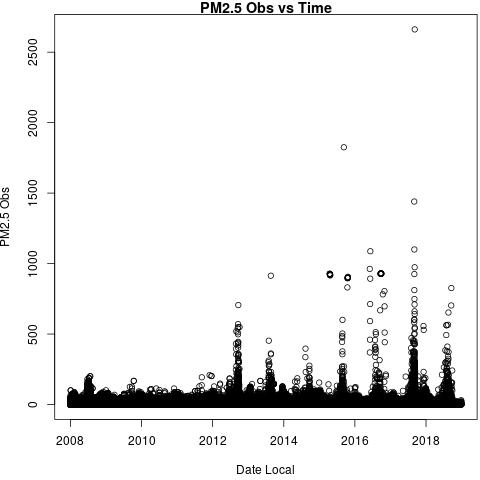
\includegraphics[width=0.77\textwidth]{Code_Outputs/Report_PM25_Step4_part_e_de_duplicated_aves_ML_input_PM25_ObsvDate_Local.jpg} 
\caption{\label{fig:Report_PM25_Step4_part_e_de_duplicated_aves_ML_inputPM25_ObsvDate_Local}vs Time} 
\end{figure} 
 

\begin{figure} 
\centering  
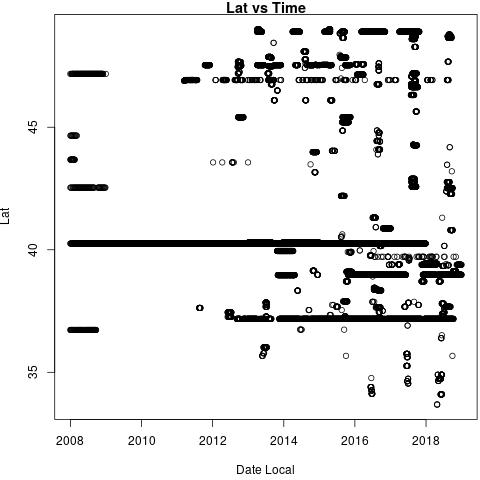
\includegraphics[width=0.77\textwidth]{Code_Outputs/Report_PM25_Step4_part_e_de_duplicated_aves_ML_input_LatvDate_Local.jpg} 
\caption{\label{fig:Report_PM25_Step4_part_e_de_duplicated_aves_ML_inputLatvDate_Local}vs Time} 
\end{figure} 
 

\begin{figure} 
\centering  
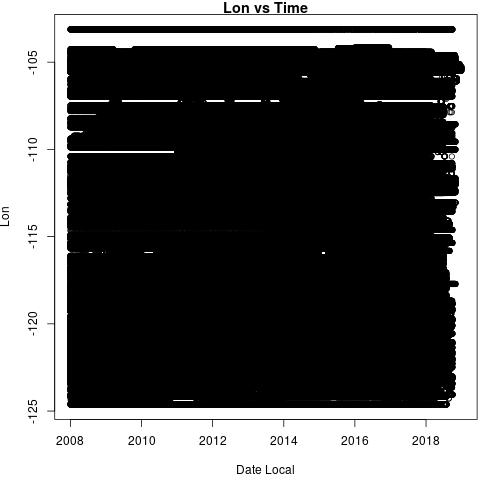
\includegraphics[width=0.77\textwidth]{Code_Outputs/Report_PM25_Step4_part_e_de_duplicated_aves_ML_input_LonvDate_Local.jpg} 
\caption{\label{fig:Report_PM25_Step4_part_e_de_duplicated_aves_ML_inputLonvDate_Local}vs Time} 
\end{figure} 
 

\begin{figure} 
\centering  
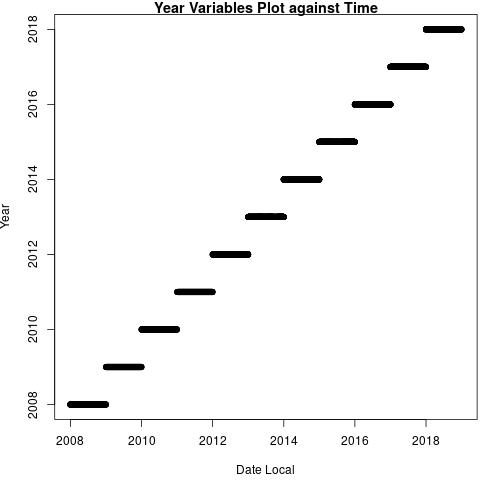
\includegraphics[width=0.77\textwidth]{Code_Outputs/Report_PM25_Step4_part_e_de_duplicated_aves_ML_input_YearvDate_Local.jpg} 
\caption{\label{fig:Report_PM25_Step4_part_e_de_duplicated_aves_ML_inputYearvDate_Local}vs Time} 
\end{figure} 
 

\begin{figure} 
\centering  
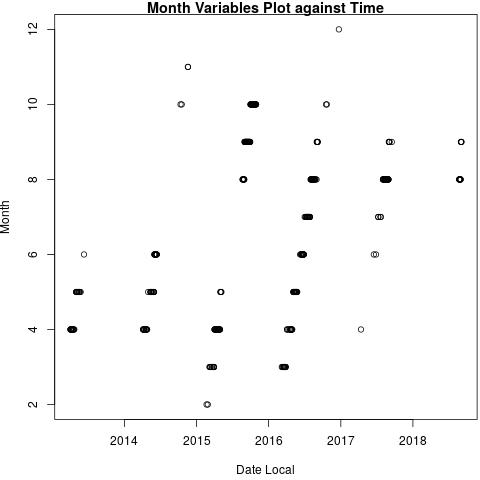
\includegraphics[width=0.77\textwidth]{Code_Outputs/Report_PM25_Step4_part_e_de_duplicated_aves_ML_input_MonthvDate_Local.jpg} 
\caption{\label{fig:Report_PM25_Step4_part_e_de_duplicated_aves_ML_inputMonthvDate_Local}vs Time} 
\end{figure} 
 

\begin{figure} 
\centering  
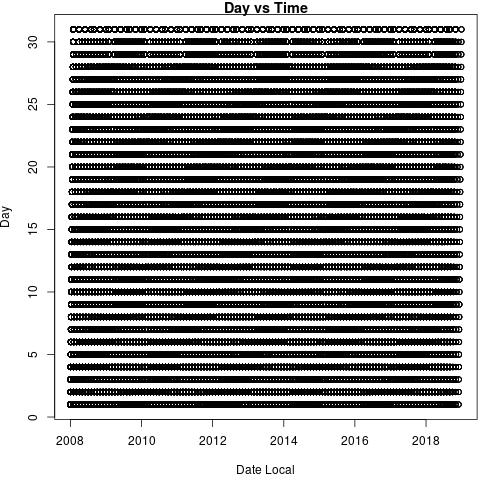
\includegraphics[width=0.77\textwidth]{Code_Outputs/Report_PM25_Step4_part_e_de_duplicated_aves_ML_input_DayvDate_Local.jpg} 
\caption{\label{fig:Report_PM25_Step4_part_e_de_duplicated_aves_ML_inputDayvDate_Local}vs Time} 
\end{figure} 
 

\begin{figure} 
\centering  
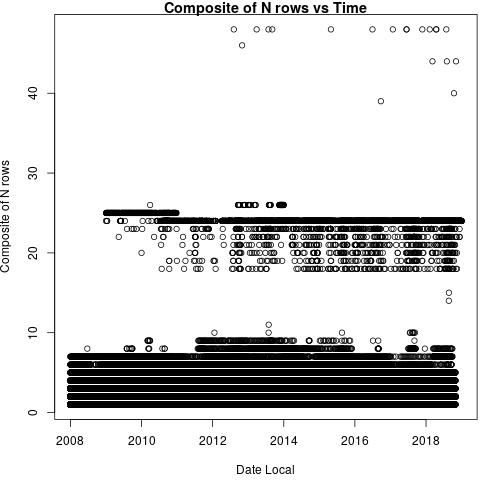
\includegraphics[width=0.77\textwidth]{Code_Outputs/Report_PM25_Step4_part_e_de_duplicated_aves_ML_input_Composite_of_N_rowsvDate_Local.jpg} 
\caption{\label{fig:Report_PM25_Step4_part_e_de_duplicated_aves_ML_inputComposite_of_N_rowsvDate_Local}vs Time} 
\end{figure} 
 

\begin{figure} 
\centering  
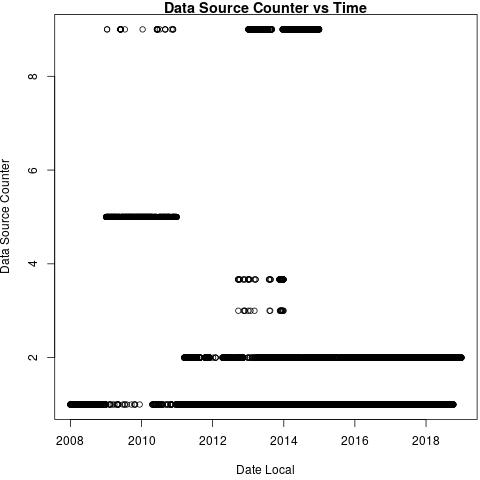
\includegraphics[width=0.77\textwidth]{Code_Outputs/Report_PM25_Step4_part_e_de_duplicated_aves_ML_input_Data_Source_CountervDate_Local.jpg} 
\caption{\label{fig:Report_PM25_Step4_part_e_de_duplicated_aves_ML_inputData_Source_CountervDate_Local}vs Time} 
\end{figure} 
 

\begin{figure} 
\centering  
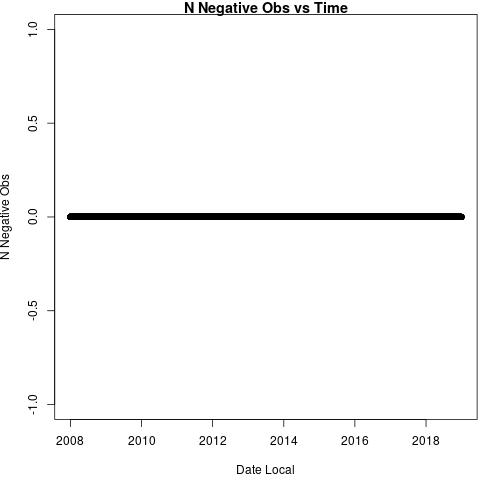
\includegraphics[width=0.77\textwidth]{Code_Outputs/Report_PM25_Step4_part_e_de_duplicated_aves_ML_input_N_Negative_ObsvDate_Local.jpg} 
\caption{\label{fig:Report_PM25_Step4_part_e_de_duplicated_aves_ML_inputN_Negative_ObsvDate_Local}vs Time} 
\end{figure} 
 

\clearpage 

\begin{figure} 
\centering  
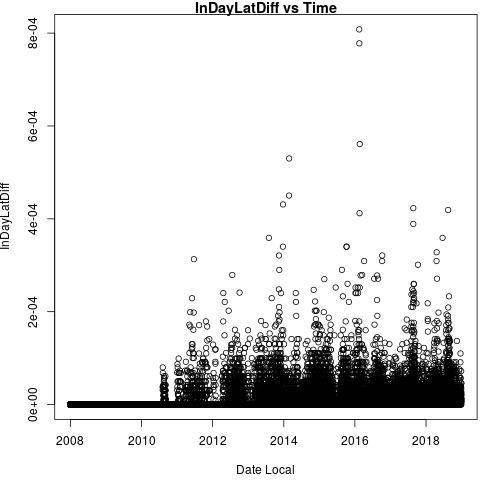
\includegraphics[width=0.77\textwidth]{Code_Outputs/Report_PM25_Step4_part_e_de_duplicated_aves_ML_input_InDayLatDiffvDate_Local.jpg} 
\caption{\label{fig:Report_PM25_Step4_part_e_de_duplicated_aves_ML_inputInDayLatDiffvDate_Local}vs Time} 
\end{figure} 
 

\begin{figure} 
\centering  
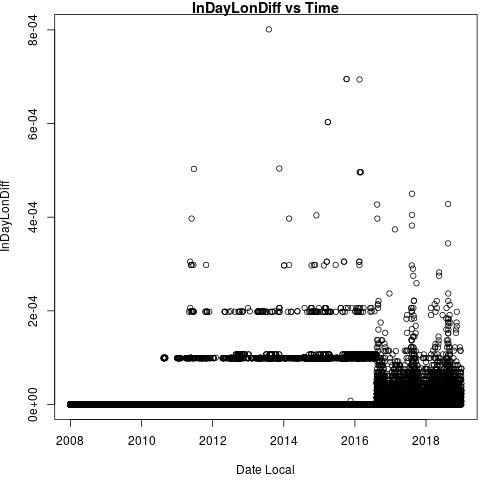
\includegraphics[width=0.77\textwidth]{Code_Outputs/Report_PM25_Step4_part_e_de_duplicated_aves_ML_input_InDayLonDiffvDate_Local.jpg} 
\caption{\label{fig:Report_PM25_Step4_part_e_de_duplicated_aves_ML_inputInDayLonDiffvDate_Local}vs Time} 
\end{figure} 
 

\subsection{All PM2.5 Monitor Locations Images} 
 

\begin{figure} 
\centering  
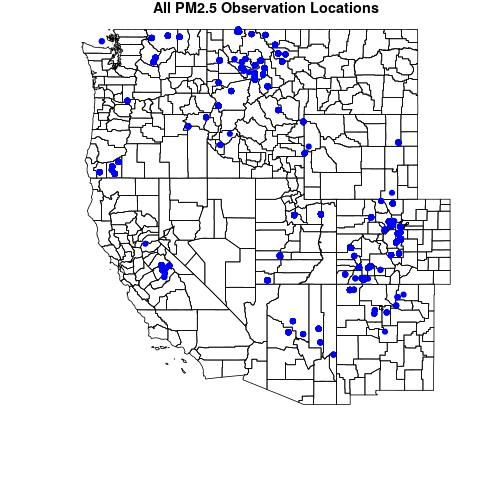
\includegraphics[width=0.77\textwidth]{Code_Outputs/Report_PM25_Step4_part_e_de_duplicated_aves_ML_input_PlotLoc0.jpg} 
\caption{\label{fig:Report_PM25_Step4_part_e_de_duplicated_aves_ML_inputPlotLoc0}All PM2.5 Observation Locations} 
\end{figure} 
 

\begin{figure} 
\centering  
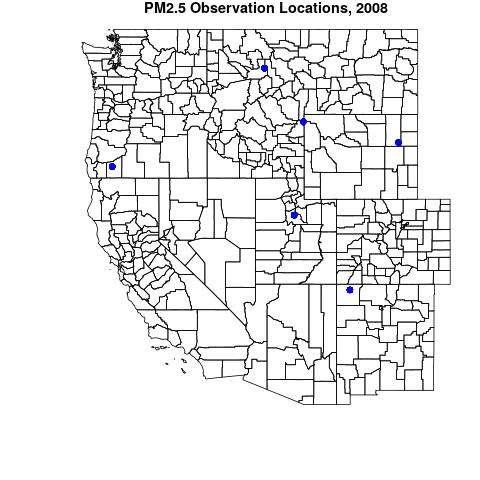
\includegraphics[width=0.77\textwidth]{Code_Outputs/Report_PM25_Step4_part_e_de_duplicated_aves_ML_input_PlotLoc2008.jpg} 
\caption{\label{fig:Report_PM25_Step4_part_e_de_duplicated_aves_ML_inputPlotLoc2008}PM2.5 Observation Locations, 2008} 
\end{figure} 
 

\begin{figure} 
\centering  
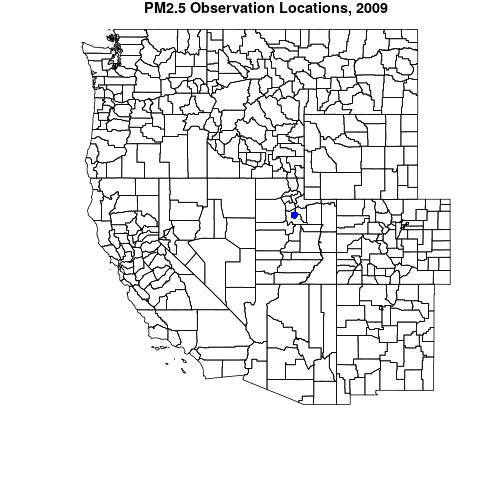
\includegraphics[width=0.77\textwidth]{Code_Outputs/Report_PM25_Step4_part_e_de_duplicated_aves_ML_input_PlotLoc2009.jpg} 
\caption{\label{fig:Report_PM25_Step4_part_e_de_duplicated_aves_ML_inputPlotLoc2009}PM2.5 Observation Locations, 2009} 
\end{figure} 
 

\begin{figure} 
\centering  
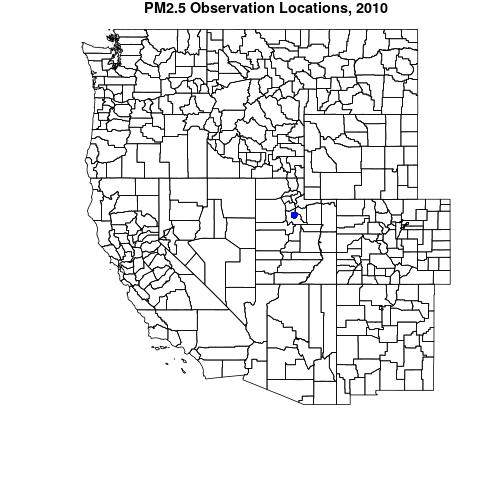
\includegraphics[width=0.77\textwidth]{Code_Outputs/Report_PM25_Step4_part_e_de_duplicated_aves_ML_input_PlotLoc2010.jpg} 
\caption{\label{fig:Report_PM25_Step4_part_e_de_duplicated_aves_ML_inputPlotLoc2010}PM2.5 Observation Locations, 2010} 
\end{figure} 
 

\begin{figure} 
\centering  
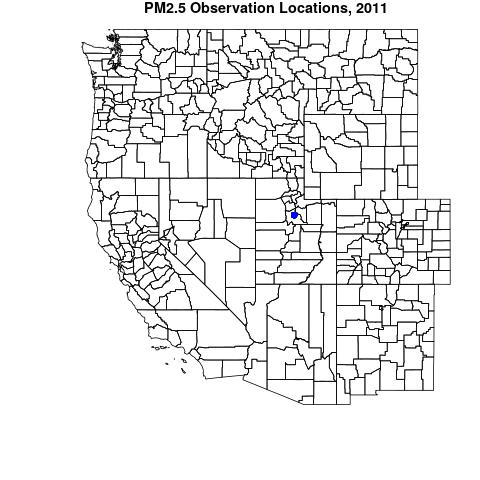
\includegraphics[width=0.77\textwidth]{Code_Outputs/Report_PM25_Step4_part_e_de_duplicated_aves_ML_input_PlotLoc2011.jpg} 
\caption{\label{fig:Report_PM25_Step4_part_e_de_duplicated_aves_ML_inputPlotLoc2011}PM2.5 Observation Locations, 2011} 
\end{figure} 
 

\begin{figure} 
\centering  
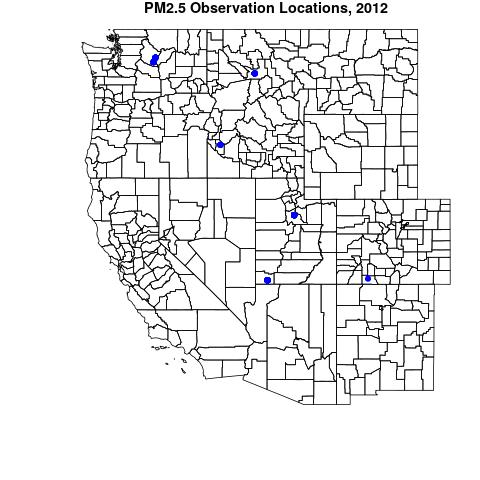
\includegraphics[width=0.77\textwidth]{Code_Outputs/Report_PM25_Step4_part_e_de_duplicated_aves_ML_input_PlotLoc2012.jpg} 
\caption{\label{fig:Report_PM25_Step4_part_e_de_duplicated_aves_ML_inputPlotLoc2012}PM2.5 Observation Locations, 2012} 
\end{figure} 
 

\begin{figure} 
\centering  
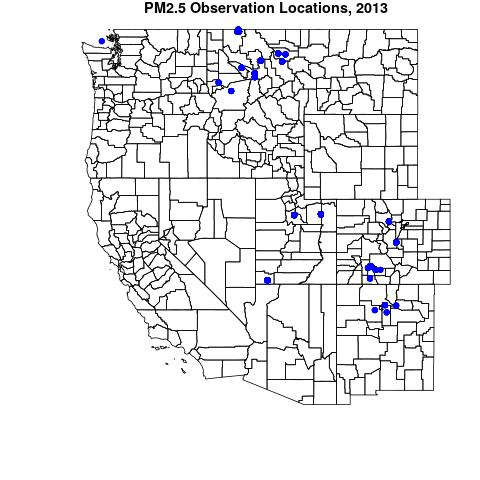
\includegraphics[width=0.77\textwidth]{Code_Outputs/Report_PM25_Step4_part_e_de_duplicated_aves_ML_input_PlotLoc2013.jpg} 
\caption{\label{fig:Report_PM25_Step4_part_e_de_duplicated_aves_ML_inputPlotLoc2013}PM2.5 Observation Locations, 2013} 
\end{figure} 
 

\begin{figure} 
\centering  
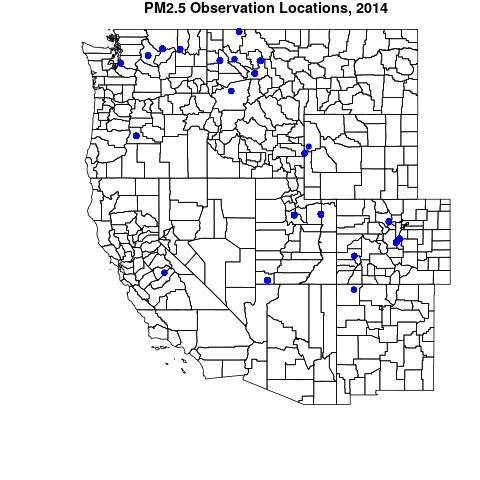
\includegraphics[width=0.77\textwidth]{Code_Outputs/Report_PM25_Step4_part_e_de_duplicated_aves_ML_input_PlotLoc2014.jpg} 
\caption{\label{fig:Report_PM25_Step4_part_e_de_duplicated_aves_ML_inputPlotLoc2014}PM2.5 Observation Locations, 2014} 
\end{figure} 
 

\begin{figure} 
\centering  
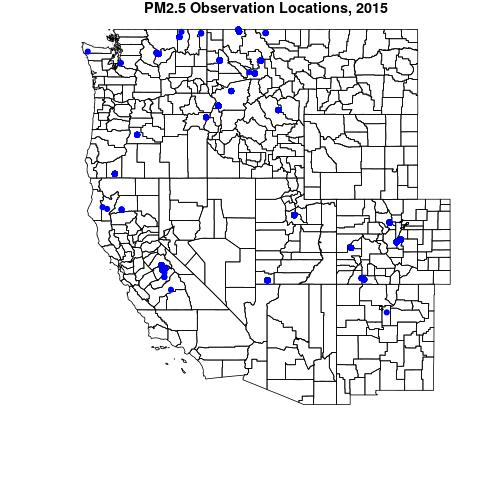
\includegraphics[width=0.77\textwidth]{Code_Outputs/Report_PM25_Step4_part_e_de_duplicated_aves_ML_input_PlotLoc2015.jpg} 
\caption{\label{fig:Report_PM25_Step4_part_e_de_duplicated_aves_ML_inputPlotLoc2015}PM2.5 Observation Locations, 2015} 
\end{figure} 
 

\begin{figure} 
\centering  
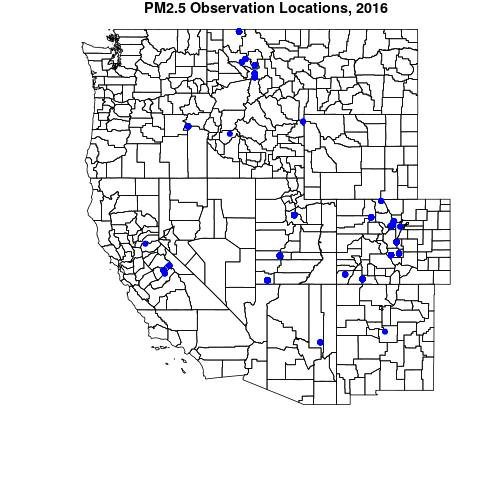
\includegraphics[width=0.77\textwidth]{Code_Outputs/Report_PM25_Step4_part_e_de_duplicated_aves_ML_input_PlotLoc2016.jpg} 
\caption{\label{fig:Report_PM25_Step4_part_e_de_duplicated_aves_ML_inputPlotLoc2016}PM2.5 Observation Locations, 2016} 
\end{figure} 
 

\begin{figure} 
\centering  
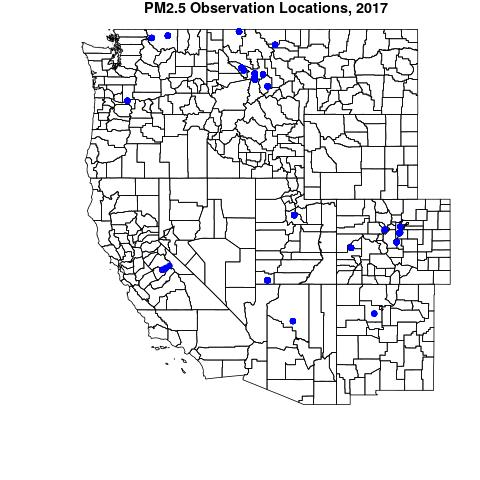
\includegraphics[width=0.77\textwidth]{Code_Outputs/Report_PM25_Step4_part_e_de_duplicated_aves_ML_input_PlotLoc2017.jpg} 
\caption{\label{fig:Report_PM25_Step4_part_e_de_duplicated_aves_ML_inputPlotLoc2017}PM2.5 Observation Locations, 2017} 
\end{figure} 
 

\begin{figure} 
\centering  
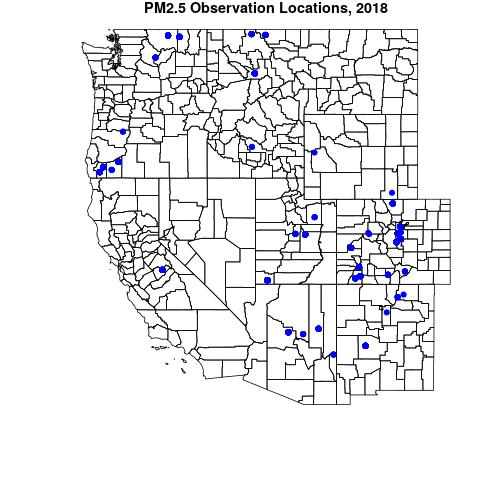
\includegraphics[width=0.77\textwidth]{Code_Outputs/Report_PM25_Step4_part_e_de_duplicated_aves_ML_input_PlotLoc2018.jpg} 
\caption{\label{fig:Report_PM25_Step4_part_e_de_duplicated_aves_ML_inputPlotLoc2018}PM2.5 Observation Locations, 2018} 
\end{figure} 
 
 % UNCOMMENT

\end{document}



